\documentclass[twocolumn, a4paper, polish, 10pt]{article}
\usepackage[polish]{babel}
\usepackage[T1]{fontenc}
\usepackage{secdot}
\usepackage{indentfirst}
\usepackage{graphicx}
\usepackage{titlesec}
\usepackage[dvipsnames,svgnames,table]{xcolor}
\definecolor{fiolet}{cmyk}{0.47,1,0.07,0.33}
\usepackage[a4paper, hmargin=2cm, tmargin=1.5cm, bmargin=3cm, footskip=2cm]{geometry}
\usepackage{fancyhdr}

% Additional imports
\usepackage{xurl}
\usepackage{hyperref}
\usepackage{amsmath}
\usepackage{amssymb}
\usepackage{physics}
\usepackage{microtype}
\usepackage[colorinlistoftodos]{todonotes}
\usepackage{tikz}
\usepackage{pgfplots}
\usepackage{csquotes}

\hypersetup{
    colorlinks=true,
    linkcolor=black,
    urlcolor=blue,
    citecolor=blue
}
\setlength {\marginparwidth }{2cm}
\pgfplotsset{compat=1.18}

\pagestyle{fancy}
\lhead{}
\chead{}
\rhead{}
\cfoot{}
\rfoot{\emph{Paweł~Konopka}}
\renewcommand{\headrulewidth}{0pt}
\renewcommand{\thefootnote}{\fnsymbol{footnote}}
\cfoot{\thepage{}}

\newcommand{\Tp}{\ensuremath{ T_{\mathrm{p}} }}
\newcommand{\Tk}{\ensuremath{ T_{\mathrm{k}} }}

\newcommand{\mK}{\ensuremath{ m_{\mathrm{k}} }}
\newcommand{\mW}{\ensuremath{ m_{\mathrm{w}} }}
\newcommand{\mL}{\ensuremath{ m_{\mathrm{l}} }}

\newcommand{\mKW}{\ensuremath{ m_{\mathrm{k+w}} }}
\newcommand{\mKWL}{\ensuremath{ m_{\mathrm{k+w+l}} }}

\newcommand{\cW}{\ensuremath{ c_{\mathrm{w}} }}
\newcommand{\cK}{\ensuremath{ c_{\mathrm{k}} }}
\newcommand{\qT}{\ensuremath{ q_{\mathrm{t}} }}

\newcommand{\degCel}{\ensuremath{ \mathrm{^{\circ}C} }}


\begin{document}

\titleformat*{\section}{\large\bfseries\centering}
\titleformat*{\subsection}{\normalsize\bfseries}
\titleformat*{\subsubsection}{\small\bfseries}

\twocolumn[
\begin{@twocolumnfalse}
\begin{center}
\textbf{\large{Wyznaczanie ciepła topnienia lodu}}
\bigskip
\\inż.~Paweł~Konopka\footnotemark \\ \small{opiekun: mgr Krzysztof Prościński}\\\textit{I Pracownia Fizyczna,
Instytut Fizyki UJ}\\
\small{data rozpoczęcia ćwiczenia: 1~kwietnia~2026}\\
\end{center}

%Abstrakt
\begin{quote}\small{
\begin{quote}
\begin{center}
\textbf{Streszczenie}
\end{center}
Celem doświadczenia było wyznaczenie ciepła topnienia lodu.
W tym celu wykorzystano kalorymetr oraz bilans cieplny.
Do aluminiowego kalorymetru z letnią wodą o znanej masie i temperaturze początkowej wrzucano osuszone kawałki topniejącego lodu ($0\degCel$).
Po całkowitym stopieniu lodu i osiągnięciu stanu równowagi termicznej, mierzono temperaturę końcową układu.
Na podstawie przeprowadzonych pięciu serii pomiarowych wyznaczono średnią wartość ciepła topnienia lodu równą $\bar{\qT} = (316 \pm 16)~\mathrm{J \, g^{-1}}$. Otrzymany wynik jest o około $5\%$ mniejszy od wartości tablicowej ($332~\mathrm{J \, g^{-1}}$). Różnica ta jest nieznacznie większa od wyznaczonej niepewności granicznej (o ok. $4 \%$).
Obserwowane odchylenie od wartości teoretycznej można przypisać trudnym do całkowitego wyeliminowania błędom systematycznym, takim jak niedoskonała izolacja termiczna kalorymetru, ewentualne resztki wody na powierzchni wrzucanego lodu oraz możliwa ujemna temperatura wewnątrz grubszych bryłek.
\end{quote}
}
\end{quote}
 \bigskip
    \bigskip
\end{@twocolumnfalse}
]
\footnotetext{pawel.konopka@student.uj.edu.pl}

\section{Podstawy teoretyczne}
\subsection{Ciepło właściwe i bilans cieplny}
Zjawiska cieplne w przyrodzie ściśle wiążą się z pojęciem energii wewnętrznej, na którą składa się m.in. energia kinetyczna cząsteczek oraz energia potencjalna ich wzajemnych oddziaływań.
Gdy dwa ciała o różnych temperaturach stykają się ze sobą, następuje przepływ energii od ciała o wyższej temperaturze do ciała o niższej temperaturze.
Energię przekazywaną w ten sposób nazywamy ciepłem ($Q$)~\cite{pracownia-fizyczna-c4}.

Ilość ciepła pobranego lub oddanego przez ciało, która skutkuje zmianą jego temperatury, opisuje wzór~(\ref{eq:cieplo_wlasciwe})~\cite{pracownia-fizyczna-c4}.\begin{equation}
    Q = m c \Delta T
    \label{eq:cieplo_wlasciwe}
\end{equation}
gdzie $m$ to masa ciała, $c$ to jego ciepło właściwe, a $\Delta T$ to zmiana temperatury.

Dostarczanie ciepła nie zawsze jednak prowadzi do wzrostu temperatury układu.
W przypadku ciał krystalicznych, takich jak lód, po osiągnięciu temperatury topnienia ($0\degCel$ dla lodu), dostarczana energia zużywana jest na zmianę energii potencjalnej cząsteczek – rozerwanie wiązań i zmianę stanu skupienia.
Temperatura lodu pozostaje stała aż do całkowitego stopienia.
Dobrze tę sytuację przedstawia schemat na Rysunku~\ref{fig:krzywa_ogrzewania}.
Ciepło niezbędne do przeprowadzenia przemiany fazowej opisuje zależność~(\ref{eq:cieplo_topnienia})~\cite{pracownia-fizyczna-c4}.
\begin{equation}
    Q_{\mathrm{top}} = \mL \qT
    \label{eq:cieplo_topnienia}
\end{equation}
gdzie $\mL$ to masa topniejącego lodu, a $\qT$ to jego ciepło topnienia.

\begin{figure}[htb]
    \centering
    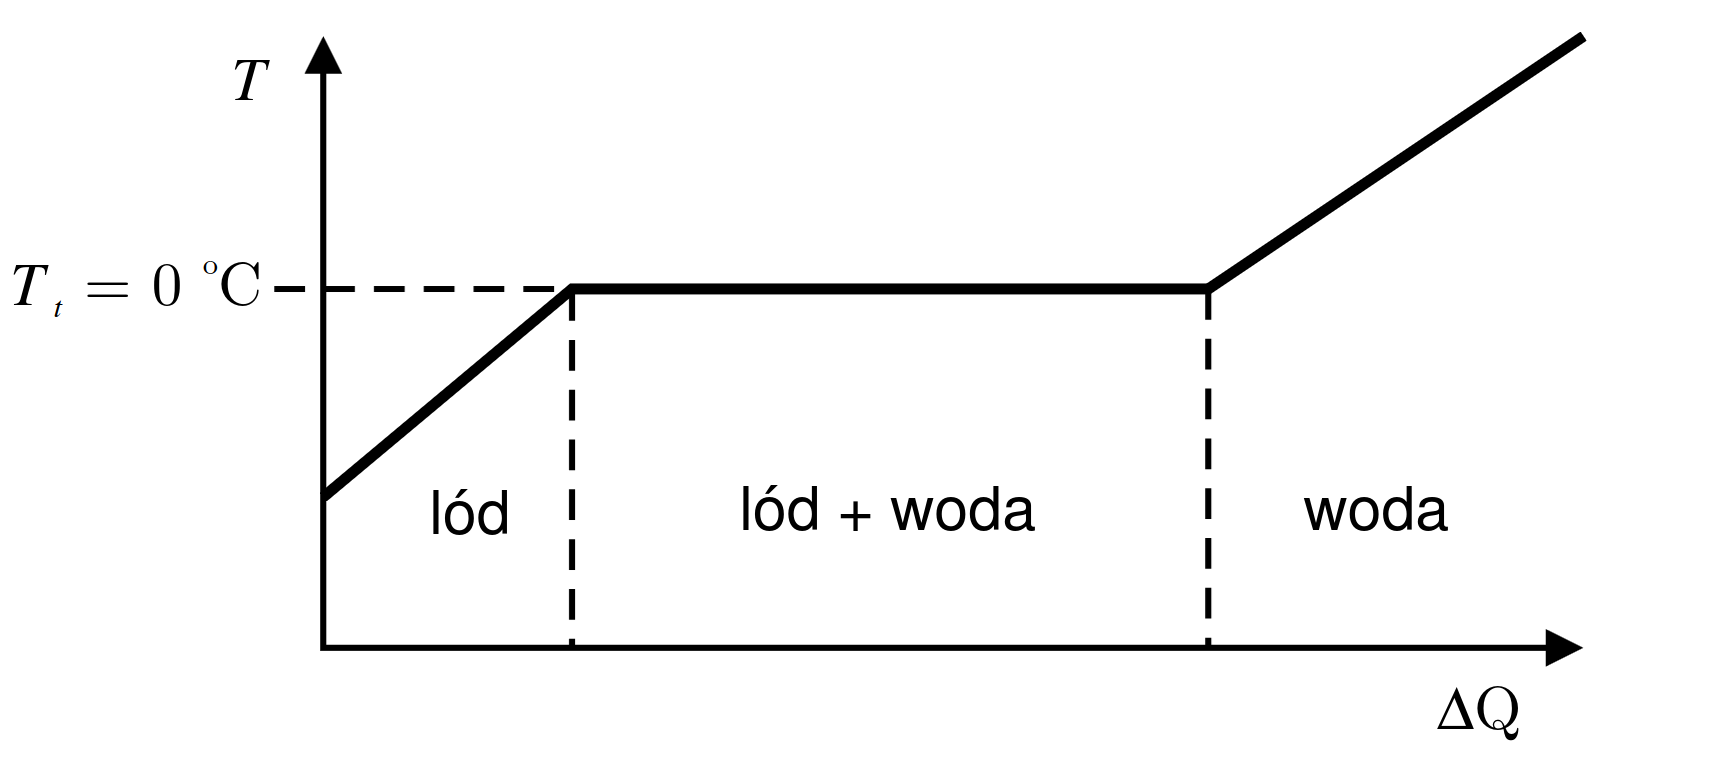
\includegraphics[width=0.9\linewidth]{img/krzywa-ogrzewania.png}
    \caption{
    Krzywa ogrzewania substancji krystalicznej.
    Źródło: I~Pracownia Fizyczna, \emph{Wyznaczanie ciepła topnienia lodu (C4)}, Instytut Fizyki~UJ~\cite{pracownia-fizyczna-c4}.
    }
    \label{fig:krzywa_ogrzewania}
\end{figure}

Zgodnie z bilansem cieplnym, w układzie izolowanym termicznie od otoczenia (np. w kalorymetrze), suma ciepła oddanego przez jedne ciała jest równa sumie ciepła pobranego przez inne.
W omawianym doświadczeniu ciepło oddaje kalorymetr (o masie $\mK$ i cieple właściwym $\cK$) oraz woda (o masie $\mW$ i cieple właściwym $\cW$), które oziębiają się z temperatury początkowej $\Tp$ do temperatury końcowej $\Tk$.
Oddane ciepło zostaje w całości zużyte na stopienie lodu o masie $\mL$ (znajdującego się w temperaturze $0\degCel$), a następnie na ogrzanie powstałej z niego wody do temperatury końcowej $\Tk$~\cite{pracownia-fizyczna-c4}.

Równanie bilansu cieplnego przyjmuje zatem postać~(\ref{eq:bilans_cieplny})~\cite{pracownia-fizyczna-c4}.
\begin{equation}
\begin{split}
    (\mW \cW + \mK \cK)(\Tp &- \Tk) = \\
    = \mL \qT &+ \mL \cW (\Tk - 0\degCel)
    \label{eq:bilans_cieplny}
\end{split}
\end{equation}

Przekształcając równanie~(\ref{eq:bilans_cieplny}), można wyznaczyć szukaną wartość ciepła topnienia lodu $\qT$ (wzór~\ref{eq:wzor_na_qt}).
\begin{equation}
    \qT = \frac{(\cW \mW + \cK \mK)(\Tp - \Tk)}{\mL} - \cW \Tk
    \label{eq:wzor_na_qt}
\end{equation}

\subsection{Ciepło właściwe wody}
Ciepło właściwe wody zależy od jej temperatury.
W temperaturach osiąganych przez nią w trakcie eksperymentu wartość ciepła właściwego zmienia się w granicach $(4.183 - 4.212)~\mathrm{\frac{J}{g~K}}$~\cite{parametry-fizyczne-wody}. Z tego względu jako $\cW$ przyjęta została wartość~(\ref{eq:cieplo-wlasciwe-wody}):
\begin{equation}
    \cW = 4.198(15)~\mathrm{\frac{J}{g \,K}}
    \label{eq:cieplo-wlasciwe-wody}
\end{equation}

\subsection{Ciepło właściwe aluminium}
Ciepło właściwe aluminium jest różne dla różnych stopów tego metalu i przyjmuje wartości w granicach $(0.856 - 0.899)~\mathrm{J \, g^{-1} \, K^{-1}}$~\cite{wlasciwosci-aluminium}.
Z tego względu jako $\cK$ przyjęta została wartość~(\ref{eq:cieplo-wlasciwe-kalorymetru}):
\begin{equation}
    \cK = 0.878(22)~\mathrm{\frac{J}{g \, K}}
    \label{eq:cieplo-wlasciwe-kalorymetru}
\end{equation}

\section{Układ pomiarowy}
Zgodnie z instrukcją do ćwiczenia, do przeprowadzenia eksperymentu wyznaczania ciepła topnienia lodu wykorzystano następujące przyrządy:
\begin{itemize}
    \item Kalorymetr pełniący funkcję naczynia izolowanego termicznie od otoczenia. Zbudowany był on z zewnętrznej obudowy izolującej oraz wewnętrznego naczynia wyposażonego w mieszadełko.
    Obie części wykonane były z aluminium i połączone przy pomocy słabo przewodzącej plastikowej części,
    \item Termometr służący do precyzyjnego pomiaru temperatury początkowej i końcowej wody wewnątrz kalorymetru,
    \item Wagę elektroniczną wykorzystywaną do wyznaczania mas poszczególnych elementów układu: pustego kalorymetru z mieszadełkiem, kalorymetru z wodą oraz kalorymetru po stopieniu lodu.
\end{itemize}

Dodatkowo, jako materiał pomocniczy w układzie pomiarowym wykorzystano ręczniki papierowe, służącą do dokładnego osuszenia bryłek lodu bezpośrednio przed ich wrzuceniem do wody w kalorymetrze.

Schematyczny rysunek układu pomiarowego analogicznego do tego wykorzystanego w doświadczeniu, przedstawiający kalorymetr wraz z zanurzonym w nim termometrem oraz mieszadełkiem, zaprezentowano na Rysunku~\ref{fig:schemat_ukladu}.

\begin{figure}[htb]
    \centering
    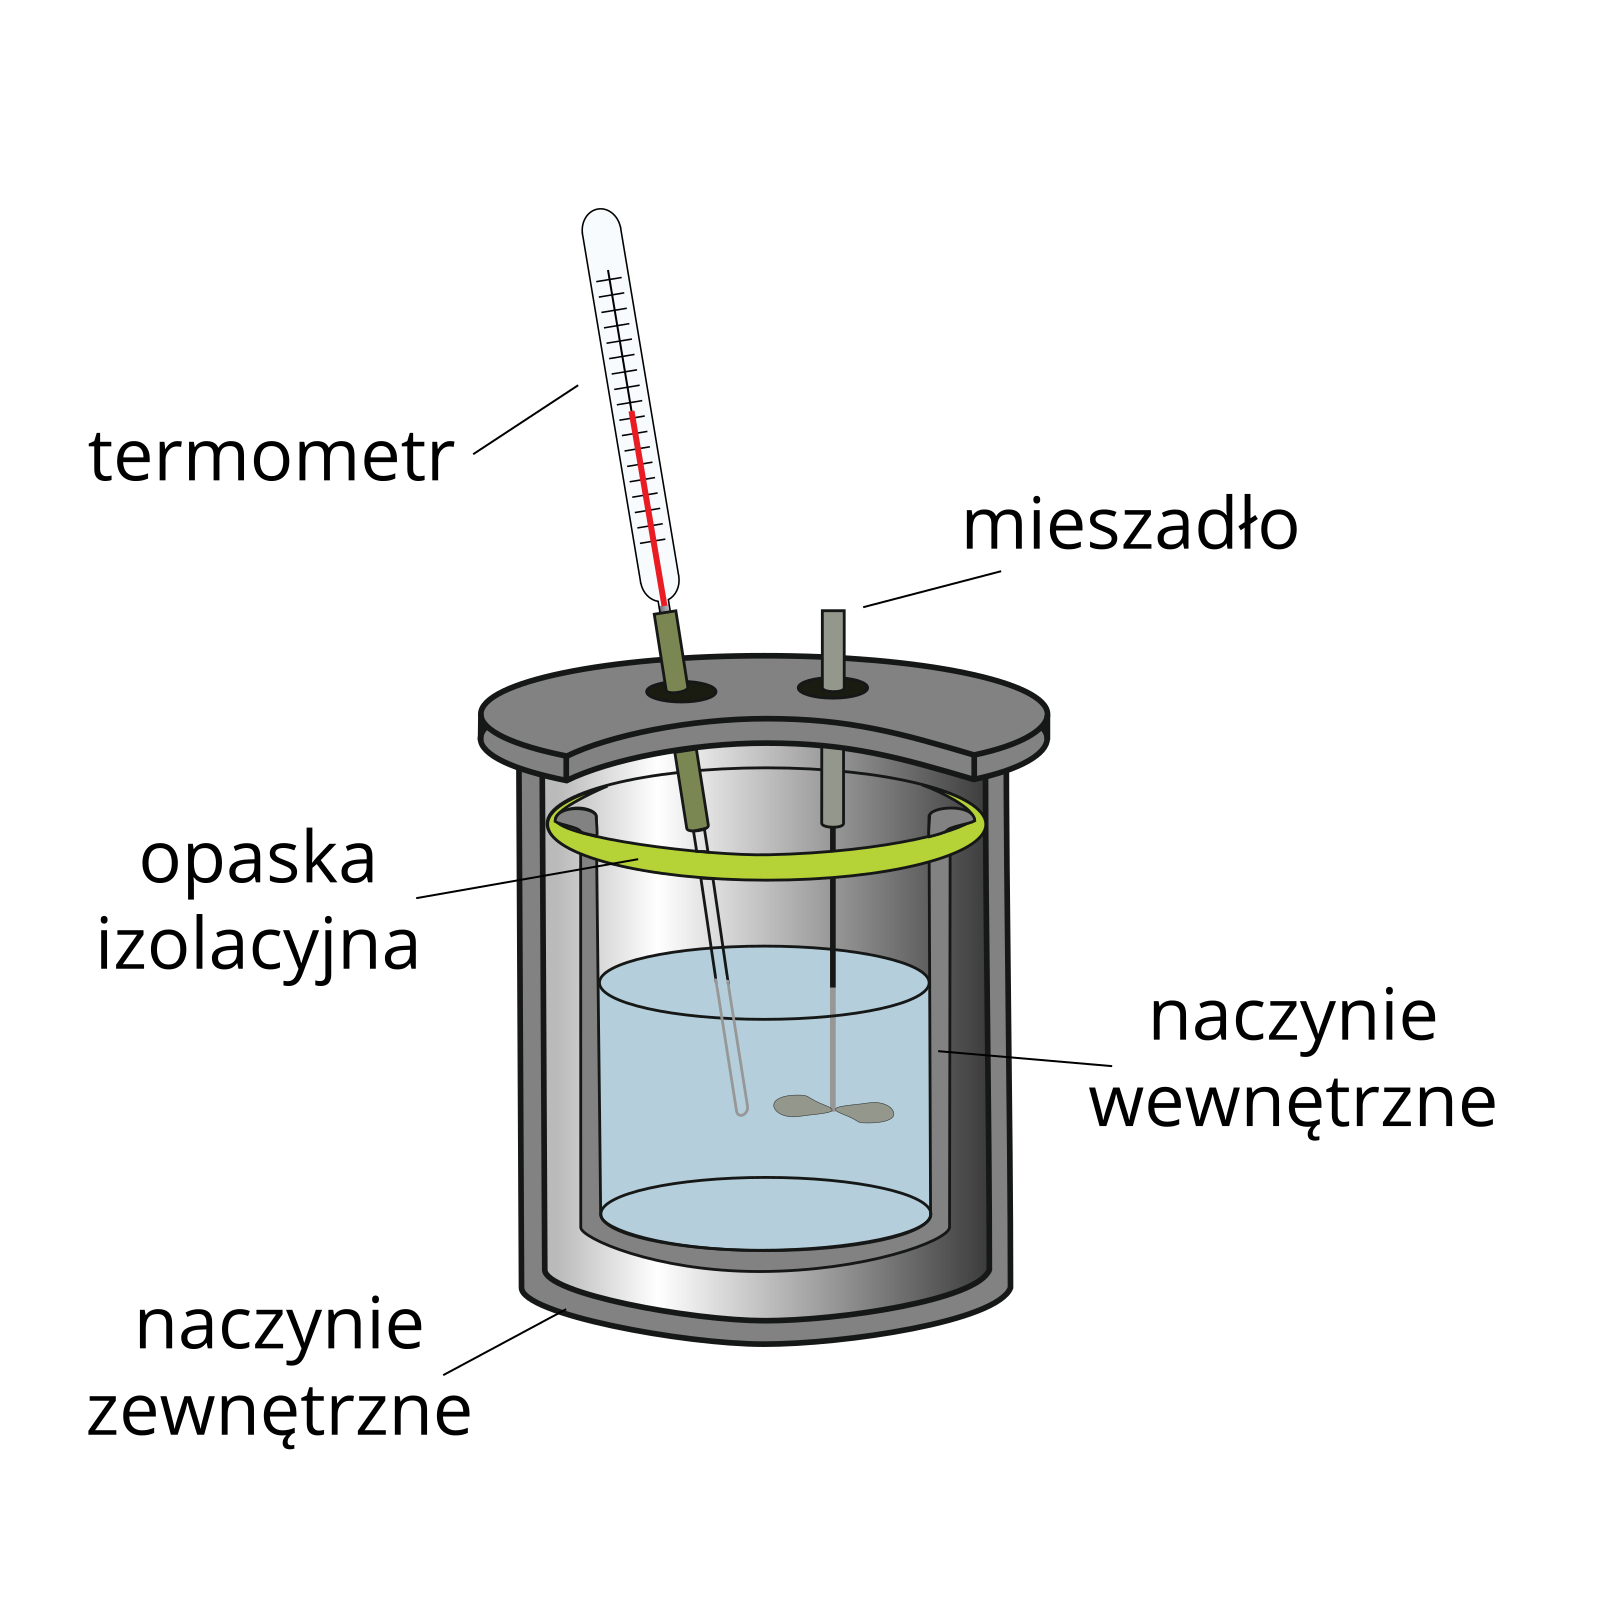
\includegraphics[width=0.8\linewidth]{img/kalorymetr-schemat.png}
    \caption{
    Schematyczny rysunek układu pomiarowego do wyznaczania ciepła topnienia lodu, składający się z kalorymetru z mieszadełkiem i termometru.
    Źródło: \emph{Zintegrowana Platforma Edukacyjna}~\cite{zpe-bilans cieplny}.
    }
    \label{fig:schemat_ukladu}
\end{figure}

\section{Przebieg pomiarów}
Pomiary rozpoczęto od sprawdzenia wypoziomowania wagi elektronicznej.
Następnie zważono wewnętrzne naczynie kalorymetru wraz z mieszadełkiem, wyznaczając w ten sposób masę pustego kalorymetru $\mK$ -- wartość~(\ref{eq:masa-kalorymetru}).
Do naczynia nalano letniej wody (o temperaturze około $21\degCel$), po czym ponownie zważono układ, aby móc obliczyć masę dodanej wody $\mW$.
Po zamknięciu kalorymetru i odczekaniu na ustabilizowanie się warunków termicznych wewnątrz naczynia, odczytano i zanotowano temperaturę początkową $\Tp$.

W międzyczasie wyjęto kostki lodu z zamrażarki i zaczekano na pojawienie się wody jako efektu topnienia.
Dawało to pewność, że temperatura całości nie powinna wynosić znacznie więcej niż $0\degCel$.
Przed wrzuceniem do kalorymetru, wybrane kawałki lodu zostały bardzo dokładnie osuszone przy pomocy ręczników papierowych.
Krok ten był niezwykle istotny, ponieważ wprowadzając do układu lód z nawet odrobiną wody w stanie ciekłym na powierzchni, ze względu na dużą wartość ciepła topnienia lodu, wprowadzono by znaczne błędy systematyczne do bilansu cieplnego~\cite{pracownia-fizyczna-c4}.

Bezpośrednio po osuszeniu, lód umieszczono w kalorymetrze. Zawartość naczynia sporadycznie delikatnie mieszano, starając się nie wykonać zbyt dużej pracy mechanicznej, jednocześnie przyspieszając osiągnięcie równowagi termicznej.
Gdy proces topnienia dobiegł końca i układ osiągnął równowagę, odczytano i zapisano temperaturę końcową mieszaniny $\Tk$.
Ostatnim krokiem w danej serii było ponowne zważenie kalorymetru z całą zawartością, co pozwoliło ustalić masę dodanego lodu $\mL$.

\subsection{Niepewności pomiarowe}
Całą opisaną powyżej procedurę powtórzono pięciokrotnie w celu zgromadzenia odpowiedniej liczby niezależnych serii pomiarowych. Temperatura początkowa wody w następnych seriach była nieco niższa niż początkowo ze względu na wychłodzenie kalorymetru.

Przed przystąpieniem do analizy zebranych danych, oszacowano niepewności graniczne pomiarów bezpośrednich na podstawie parametrów użytych przyrządów.
W przypadku wagi elektronicznej przyjęto niepewność pomiaru masy równą jej rozdzielczości, a więc wartość~(\ref{eq:niepewnosc-masy}).
\begin{equation}
    \Delta m = 0.1~\mathrm{g}
    \label{eq:niepewnosc-masy}
\end{equation}
Z kolei niepewność pomiaru temperatury wyznaczono na podstawie działki elementarnej termometru, przyjmując wartość~(\ref{eq:niepewnosc-temperatury}).
\begin{equation}
    \Delta T = 0.2\degCel
    \label{eq:niepewnosc-temperatury}
\end{equation}

Powyższe wartości przypisano do wszystkich odczytów i wykorzystano w dalszym etapie do obliczenia niepewności złożonej wyznaczanego ciepła topnienia lodu przy pomocy wzoru~(\ref{eq:propagacja-niepewnosci-wiele-zmiennych}).

\section{Wyniki i dyskusja}
Zmierzona masa pustego kalorymetru wraz z mieszadełkiem $\mK$ ma wartość~(\ref{eq:masa-kalorymetru}).
\begin{equation}
    \mK = 137.0(1)~\mathrm{g}
    \label{eq:masa-kalorymetru}
\end{equation}

Zmierzone wartości temperatur oraz mas kalorymetru wraz z wodą, oraz całości po roztopieniu lodu zaprezentowane są w Tabeli~\ref{tab:pomiary}.

\begin{table}[htb]
\begin{center}
\renewcommand*{\tablename}{Tabela}
\caption{\small
Zmierzone wartości temperatury początkowej $\Tp$, temperatury końcowej $\Tk$, masy kalorymetru z wodą $\mKW$ oraz sumarycznej masy po wrzuceniu lodu $\mKWL$ wszystkich serii pomiarowych.
\vspace{0.15cm}
    \label{tab:pomiary}}
    {\small
    \begin{tabular}{c c c c c}
    \hline \vspace{-0.35cm} \\
      Seria & $\Tp~[\degCel]$ & $\Tk~[\degCel]$
      & $\mKW~[\mathrm{g}]$ & $\mKWL~[\mathrm{g}]$ \\
      \hline \vspace{-0.2cm} \\
      1 & 21.4 & 8.8 & 560.9 & 628.3 \\
      2 & 20.5 & 7.9 & 494.5 & 552.7 \\
      3 & 20.8 & 7.0 & 581.8 & 661.4 \\
      4 & 20.6 & 6.4 & 578.9 & 663.6 \\
      5 & 20.7 & 10.2 & 633.8 & 697.2 \\
    \hline
    \end{tabular}}
    \end{center}
\end{table}


Wartości obliczone przy pomocy zależności~(\ref{eq:cieplo-wlasciwe-wody}) oraz zmierzonej wartości~(\ref{eq:masa-kalorymetru}) zaprezentowane są w Tabeli~\ref{tab:cieplo-wlasciwe}.
Każdy z pomiarów masy wody $\mW$ oraz masy lodu $\mL$ obarczony jest niepewnością graniczną: $\Delta \mW = \Delta \mL = 2 \cdot \Delta m = 0.2~\mathrm{g}$, co jest konsekwencją wzoru~(\ref{eq:propagacja-niepewnosci-wiele-zmiennych}).

\begin{table}[htb]
\begin{center}
\renewcommand*{\tablename}{Tabela}
\caption{\small
Obliczone wartości pochodne dla każdej serii pomiarowej: spadek temperatury $(-\Delta T)$, masa wody $\mW$, masa lodu $\mL$ oraz obliczone ciepło topnienia lodu $\qT$.
\vspace{0.15cm}
    \label{tab:cieplo-wlasciwe}}
    {\small
    \begin{tabular}{c c c c c}
    \hline \vspace{-0.35cm} \\
      Seria & $-\Delta T~[\degCel]$
      & $\mW~[\mathrm{g}]$ & $\mL~[\mathrm{g}]$ & $\qT~[\mathrm{J~g^{-1}}]$ \\
      \hline \vspace{-0.2cm} \\
      1 & 12.6 & 423.9 & 67.4 & 318(16) \\
      2 & 12.6 & 357.5 & 58.2 & 318(17) \\
      3 & 13.8 & 444.8 & 79.6 & 315(15) \\
      4 & 14.2 & 441.9 & 84.7 & 304(15) \\
      5 & 10.5 & 496.8 & 63.4 & 322(19) \\
    \hline
    \end{tabular}}
    \end{center}
\end{table}

Przy pomocy wartości ciepła topnienia $\qT$ dla poszczególnych serii obliczona została wartość średnia $\bar{\qT}$:
\begin{displaymath}
    \bar{\qT} = (316 \pm 16)~\mathrm{\frac{J}{g}}
\end{displaymath}

Przyglądając się uzyskanym wartościom $\qT$ z Tabeli~\ref{tab:cieplo-wlasciwe} na uwagę zasługuje zdecydowanie odstający wynik uzyskany w serii 4. Gdyby odrzucić ten wynik ze względu na możliwe wystąpienie błędu grubego otrzymalibyśmy wartość $\bar{\qT}'$:
\begin{displaymath}
    \bar{\qT}' = (318 \pm 17)~\mathrm{\frac{J}{g}}
\end{displaymath}

\section{Podsumowanie}
\subsection{Porównanie z wartością tablicową}
Wartość $\bar{\qT}$ różni się od wartości tablicowej ($q_{\mathrm{Tab}}=332~\mathrm{J~g^{-1}}$)~\cite{pracownia-fizyczna-c4} o około $5\%$, co przekłada się na około $(1.04 \cdot \Delta \qT)$. Wynik więc nie mieści się w obliczonej niepewności granicznej, lecz jedynie nieznacznie.

Porównując natomiast wartość $\bar{\qT}'$ z wartością tablicową $q_{\mathrm{Tab}}$ uzyskujemy błąd odpowiednio $4.1\%$ i $(0.84 \cdot \Delta \qT)$. Wartość $\bar{\qT}'$ jest więc bliższa wartości tablicowej, a uzyskany błąd mieści się w obliczonej niepewności granicznej.

\subsection{Dodatkowe czynniki wpływające na niepewność pomiaru}
Na ostateczny wynik oraz jego odchylenie od wartości tablicowej mogły wpłynąć również dodatkowe czynniki i błędy systematyczne, które nie zostały uwzględnione w przeprowadzonym rachunku niepewności.
Izolacja termiczna kalorymetru nie jest idealna. Przestrzeń między ściankami naczynia nie stanowi próżni, w związku z czym układ nieustannie wymieniał pewną część ciepła z otoczeniem.

Dodatkowo, w warunkach laboratoryjnych całkowite i idealne osuszenie wprowadzanych kawałków lodu jest niezwykle trudne.
Ewentualne resztki wody w stanie ciekłym, pozostające na powierzchni lodu w momencie jego ważenia i wrzucania do kalorymetru, mogły nieznacznie zaburzyć bilans cieplny.

Ostatnim istotnym czynnikiem jest potencjalnie nierównomierny rozkład temperatury wewnątrz samych bryłek lodu.
Pomimo tego, że ich zewnętrzna warstwa ulegała topnieniu (co sugerowało osiągnięcie $0\degCel$), wnętrze grubszych kostek mogło wciąż znajdować się w temperaturze ujemnej.
W konsekwencji część ciepła oddanego przez kalorymetr i wodę musiała zostać dodatkowo zużyta na ogrzanie lodu do temperatury topnienia, co mogło przełożyć się na odchylenie wyznaczonej wartości $\qT$.

\section{Materiały dodatkowe}
\subsection{Propagacja niepewności granicznej funkcji wielu zmiennych}
Niepewność granicznej wartości $Y$, będącą wartością funkcji wielu zmiennych $(X_1, X_2, \dots, X_n)$ można policzyć przy użyciu wzoru~(\ref{eq:propagacja-niepewnosci-wiele-zmiennych}) \cite{smop-wyklad}.
\begin{equation}
    \Delta Y = \sum_{i=1}^n \left|
            \pdv{Y}{X_i} \Delta X_i
        \right|
    \label{eq:propagacja-niepewnosci-wiele-zmiennych}
\end{equation}

\begin{thebibliography}{7}
    \bibitem{parametry-fizyczne-wody} Świadomy projektant, \emph{Parametry fizyczne wody w określonej temperaturze} (\url{https://swiadomyprojektant.pl/parametry-fizyczne-wody-w-okreslonej-temperaturze/}) (dostęp:~8.04.2026).

    \bibitem{wlasciwosci-aluminium} PPUH Tozamet Tomasz Wajda, \emph{Właściwości aluminium i stopów aluminium} (\url{https://emetal.eu/aluminium/wlasciwosci-aluminium-i-stopow-aluminium/}) (dostęp:~8.04.2026).

    \bibitem{smop-wyklad} dr~hab. \mbox{Katarzyna} \mbox{Gajos}, Wykład \emph{Statystyczne Metody Opracowania Pomiarów I Dla studentów fizyki}.

    \bibitem{pracownia-fizyczna-c4} I~Pracownia Fizyczna, Instytut Fizyki~UJ, \emph{Wyznaczanie ciepła topnienia lodu (C4)} (\url{https://1pf.if.uj.edu.pl/materialy-do-cwiczen/spis-cwiczen}) (dostęp:~10.04.2026).

    \bibitem{zpe-bilans cieplny} Zintegrowana Platforma Edukacyjna, \emph{Do czego w praktyce przydaje się bilans cieplny} (\url{https://zpe.gov.pl/b/do-czego-w-praktyce-przydaje-sie-bilans-cieplny/P7YCgIZwM}) (dostęp:~11.04.2026).
\end{thebibliography}


\end{document}
